\documentclass[11pt, english]{article}
%\usepackage[latin1]{inputenc}
\usepackage[T1]{fontenc}
\usepackage[utf8]{inputenc}
\usepackage[english]{babel}   % S P R A A K


% \usepackage{graphicx}    % postscript graphics
\usepackage{amssymb, amsmath, amsthm, amssymb} % symboler, osv
\usepackage{mathrsfs}
\usepackage{url}
\usepackage{thmtools}
\usepackage{enumerate}  % lister $  
\usepackage{float}
\usepackage{tikz}
\usetikzlibrary{calc}
\usepackage{tikz-3dplot}
\usepackage{subcaption}
\usepackage[all]{xy}   % for comm.diagram
\usepackage{wrapfig} % for float right
\usepackage{hyperref}
\usepackage{mystyle} % stilfilen      

\usepackage[a5paper,margin=0.5in]{geometry}

\begin{document}
\title{Calabi-Yau hypersurface and mirror symmetry}
\author{Fredrik Meyer}
\maketitle 

\section{Preliminaries}
\begin{enumerate}
\item Stanley-Reisner schemes
\item Deformations of Stanley-Reisner schemes
\item Refer to mirror pdf for defs
\end{enumerate}

\section{The deformation}

\subsection{The Stanley-Reisner scheme $\K$}
Let $D_6$ be a hexagon, and define $\K := D_6 \ast D_6$ and let $\PP(\K)$ be the associated Stanley-Reisner scheme together with its embedding in $\PP^{11}$. We will study the deformation theory of $\K$ in some detail.

Denote the vertices of the ``left'' $D_6$ by $y_1,\cdots,y_6$ and the vertices of right one by $z_1,\cdots,z_6$.

\begin{lemma}
The automorphism group of $\K$ is $G := D_6 \times D_6 \times \Z/2$ of order $288$. There are interesting subgroups $G' := \Z/6 \times \Z/6 \times \Z/2$ and $G'' := \Z/6 \times \Z/6$.
\end{lemma}

\begin{prop}
\label{t1}
The module $T^1_0$ is $84$-dimensional. The deformations come in three types.

We have $12$ weights of type
$$
t_{i} := \frac{y_i}{y_{i+1}y_{i-1}},
$$
one for each vertex of $\K$.

There are $72$ more weights:
$$
t^{ij}_{i+1,i-1}=\frac{y_iy_j}{y_{i+1}y_{i-1}} \qquad t^{ij}_{j+1,j-1}=\frac{y_iy_j}{y_{j+1}y_{j-1}}.
$$
The module $T^1_{-1}$ is $12$-dimensional, they all have the form
$$
s_i := \frac{y_i}{y_{i+1}y_{i-1}}.
$$
\end{prop}

It follows that $K'= \K \ast \{ v \}$ has $\dim_k T^1_0 = 96$. 

\subsection{Smoothing}

Let $dP$ be the polytope associated to the del Pezzo surface of degree $6$. See Figure 1.

\begin{figure}
\label{fig:hexagon}
\centering
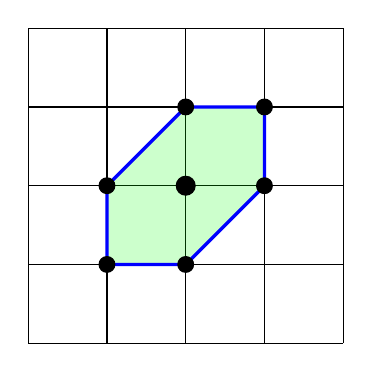
\begin{tikzpicture}
  \draw (0, 0) grid (4, 4);  

\draw [very thick, color=blue, fill=green, fill opacity=0.2]
(1,1) -- (2,1) -- (3,2) -- (3,3) -- (2,3) -- (1,2) -- cycle;

\draw [fill=black]  (1, 1) circle (0.1);
\draw [fill=black]  (2, 1) circle (0.1);
\draw [fill=black]  (3, 2) circle (0.1);
\draw [fill=black]  (3, 3) circle (0.1);
\draw [fill=black]  (2, 3) circle (0.1);
\draw [fill=black]  (1, 2) circle (0.1);
\draw [fill=black]  (2, 2) circle (0.12);


\end{tikzpicture}
\caption{The hexagon, a.k.a the polytope associated to a degree 6 del Pezzo surface.}
\end{figure}

\begin{prop}
There is a flat deformation of $\PP(\K')$ to the toric variety associated to the polar dual $(dP \times dP)^\circ$. The base space is $8$-dimensional.
\end{prop}
\begin{remark}
This is the same as $h^{12}$ of the corresponding Calabi-Yau hypersurface. This suggests that we have captured at least an open subset of the moduli space.
\end{remark}

The parameters used are all of the form $t_i$ in the notation of Proposition \ref{t1}.

\begin{corr}
There is a flat deformation of $D_6 \ast D_6$ to a singular Calabi-Yau threefold $X_t$. It has $48$ isolated singularities.

A computation in \verb|M2| shows that $X_t$ have $\dim_k T^1=96$. In particular, $X_t$ have no ordinary double points as singularities (these have $\dim_k T^1=1$).
\end{corr}

\begin{prop}
$X_t$ have canonical but not terminal singularities.
\end{prop}
\begin{proof}
Every hypersurface in a Fano toric variety have at most Gorenstein canonical singularities, by Theorem 4.19 in \cite{batyrev_dualpolyhedra} and the remarks in Section 1 in \cite{batyrev_conifoldegen}, which says that the singularities in the toric stratum $X_\theta$ are terminal if and only if the only lattice points in the dual face $\theta^\circ$ are its vertices. However, in our case, the dual polyhedron have faces with two interior points.
\end{proof}

\bibliographystyle{plain} 
\bibliography{bibliografi} 

\end{document}
